\chapter{Analyse et spécification des besoins}

\section*{Introduction}
Dans toute application informatique, les fonctionnalités doivent être mises en relation avec un ensemble de besoins définis par l'utilisateur du système. Les fonctions que le système est appelé à accomplir découlent essentiellement des besoins exprimés. La spécification des besoins constitue l'élément de base sur lequel sera construite l’architecture du système. Nous commencerons par identifier les acteurs du système. Nous définirons ensuite les besoins exprimés par ces derniers, et à partir desquels serons définis les cas d’utilisations de l'application.
%Dans ce chapitre nous nous intéressons par la phase spécification et analyse des besoins qui représente la base de départ de notre travail. Notre objectif ici est de dégager les différents acteurs ainsi que de spécifier et analyser les besoins fonctionnels et non fonctionnels relatifs au système. Nous finissons par présenter quelques diagrammes de cas d’utilisation afin d’expliquer approfondissement les besoins.
%%%%%%%%%%%%%%%%%%%%%%%%%%%%%%%%%%%%%%%%%%%%%%%%%%%%%%%%%%%
\section{Identification des acteurs}
Un acteur est l'idéalisation d'un rôle joué par une entité distincte du système et qui interagit directement avec lui. Notre module comporte deux acteurs majeurs:
 \begin{itemize} 
    \item  \textbf{ Le Back-office} : cet acteur est responsable de la gestion de la fiche du candidat et de l'assignation d'un entretien à un recruteur.
    \item  \textbf{Le recruteur} : c'est celui qui va passer l'entretien d'embauche au candidat.
 \end{itemize}
%%%%%%%%%%%%%%%%%%%%%%%%%%%%%%%%%%%%%%%%%%%%%%%%%%%%%%%%%%%
\section{Identification des besoins}
L’application offre à chaque acteur un ensemble de fonctionnalités. Cette partie sera donc consacrée aux besoins fonctionnels et non fonctionnels relatifs à l’application.
%%%%%%%%%%%%%%%%%%%%%%%%%%%%%%%%%%%%%%%%%%%%%%%%%%%%%%%%%%%
\subsection{Les besoins fonctionnels}
Dans cette partie, nous citons les fonctionnalités pour chaque acteur.
\begin{itemize}
    \item [•]Pour le back-office, l'application doit lui permettre de:   
 \begin{itemize}
     \item Gérer une fiche candidat : le back-office peut ajouter ou modifier une fiche candidat.
     \item Gérer un entretien : le back-office peut planifier un entretien, modifier certains de ses éléments ou consulter son Workflow(historique).
     \item Rechercher un candidat : le back-office peut rechercher un candidat selon plusieurs critères. 
     \item Consulter le KPI des avis des entretiens : le back-office peut consulter le graphe(en secteurs) qui indique le nombre total,par année, de candidats correspondant à chacun des avis listés.
 \end{itemize}
    \item [•] Pour le recruteur , l'application doit lui permettre de : 
 \begin{itemize}
     \item Modifier un entretien : le recruteur peut modifier certains éléments de l'entretien.
     \item Rechercher un candidat : le recruteur peut rechercher un candidat selon plusieurs critères.
     \item Valider un entretien : le recruteur peut accepter ou rejeter un entretien selon sa disponibilité.
     \item Consulter le KPI des avis des entretiens : le recruteur peut consulter le graphe(en secteurs) qui indique le nombre total,par année, de candidats correspondant à chacun des avis listés.
 \end{itemize}
\end{itemize}


%%%%%%%%%%%%%%%%%%%%%%%%%%%%%%%%%%%%%%%%%%%%%%%%%%%%%%%%
 \subsection{Les besoins non fonctionnels}
Dans l’intention de réussir notre tâche, l’application doit vérifier quelques propriétés et doit tenir compte de certaines contraintes et exigences:
 \begin{itemize}
     \item  \textbf{Ergonomie:} les interfaces graphiques de notre module de gestion des candidats doit avoir une ergonomie identique à celle des modules déjà migrés vers l'architecture microservices.
     \item \textbf{Sécurité:} notre application doit assurer la sécurité pour chaque authentification.
    \item \textbf{Maintenabilité:} notre module de gestion des candidats doit être évolutif et extensible.
 \end{itemize}
%%%%%%%%%%%%%%%%%%%%%%%%%%%%%%%%%%%%%%%%%%%%%%%%%%%%%%%%%
 \section{Diagramme de cas d'utilisation global}
Cette partie permet de montrer le comportement de l'application. Nous utilisons le diagramme de cas d'utilisation pour visualiser les fonctionnalités du système et les interactions entre les acteurs et le système.

La Figure \ref{fig:cas_utilisation_global} présente le diagramme des cas d'utilisation global de notre application montrant les fonctionnalités offertes pour chacun des deux principaux acteurs(back-office et recruteur).
 
 \begin{figure}[H]
     \centering
     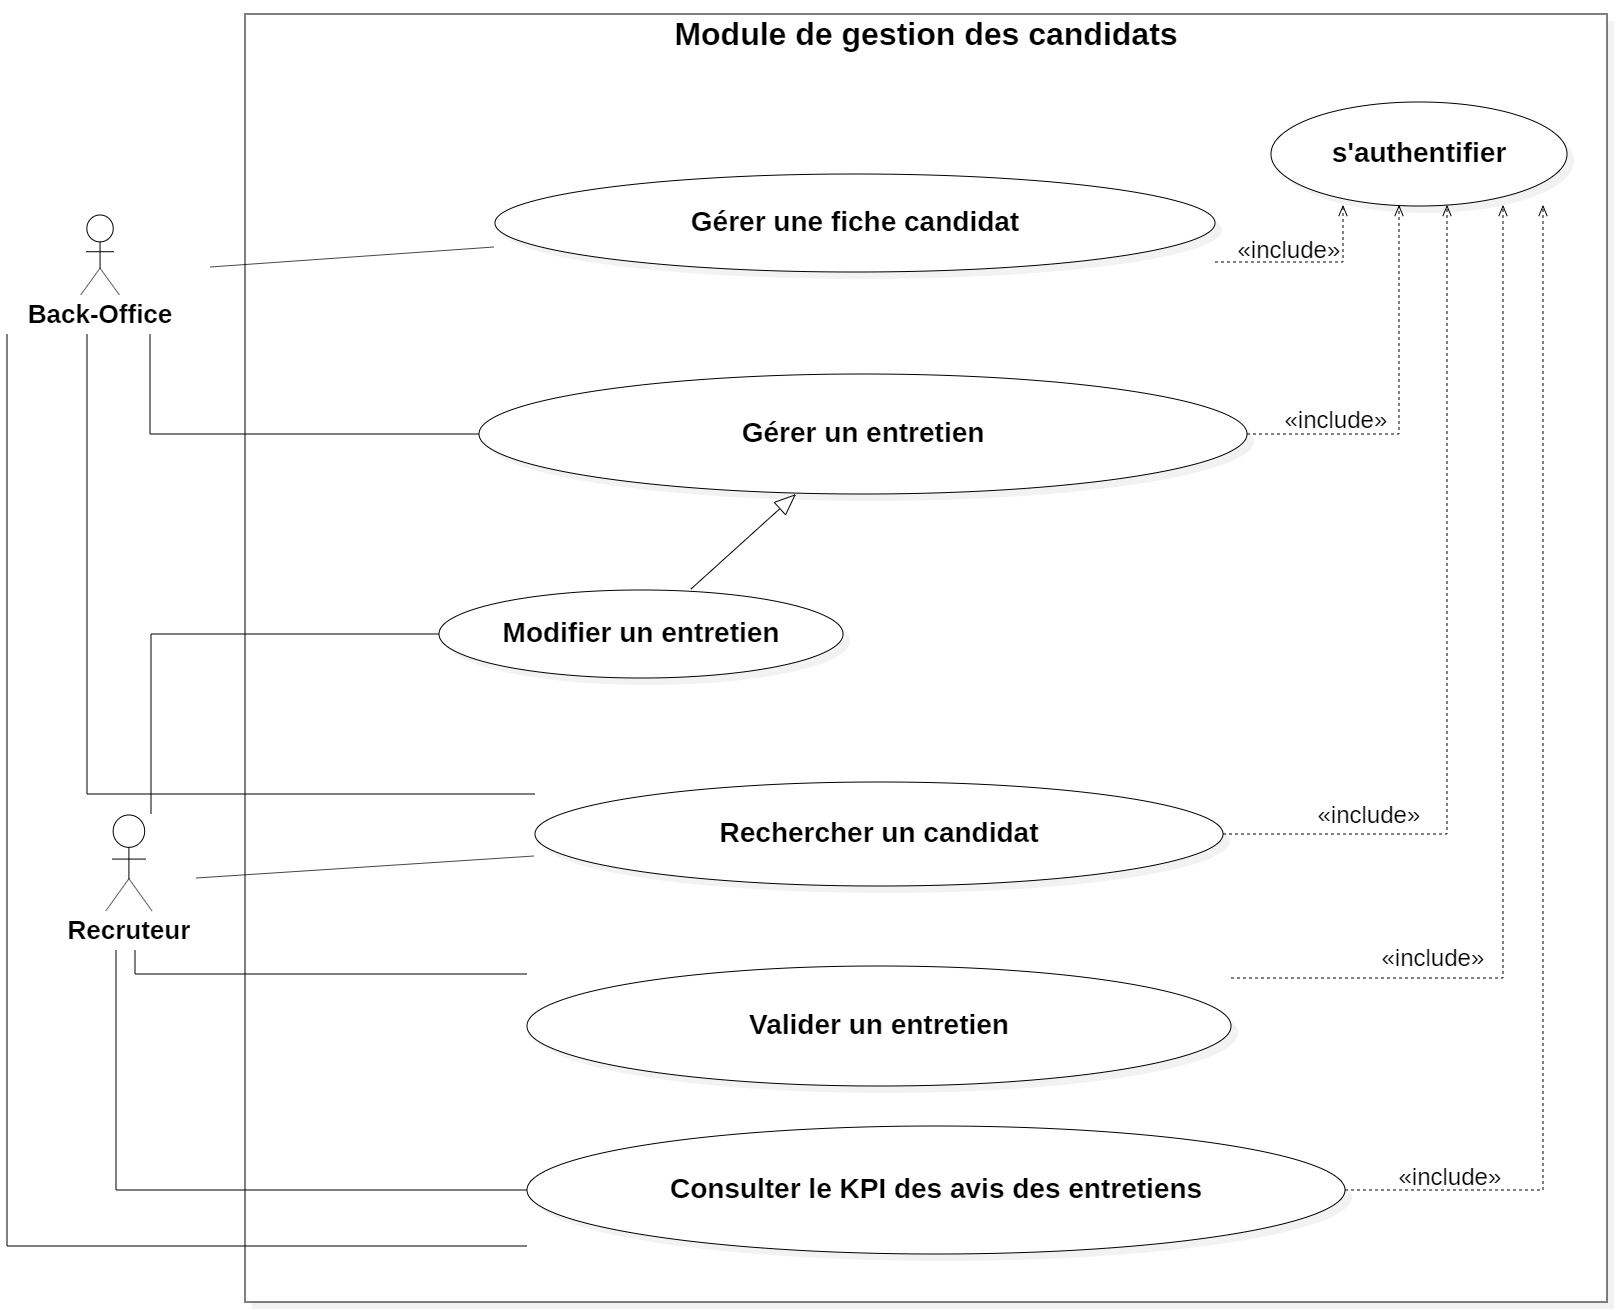
\includegraphics[scale=0.4]{img/UseCaseDiagramv4.png}
     \caption{Diagramme de cas d'utilisation global}
     \label{fig:cas_utilisation_global}
 \end{figure}
Nous présentons dans la suite le raffinement des cas d'utilisation pour chaque acteur.
%%%%%%%%%%%%%%%%%%%%%%%%%%%%%%%%%%%%%%%%%%%%%%%%%%%%%%%%
\section{Diagrammes des cas d'utilisation détaillés}
Dans cette section nous présentons, pour chaque acteur, les diagrammes des cas d'utilisation détaillés et leur description textuelle.
%%%%%%%%%%%%%%%%%%%%%%%%%%%%%%%%%%%%%%%%%%%%%%%
\subsection{Raffinement des cas d'utilisation pour le back-office}
Dans cette partie, nous développons chaque cas d'utilisation du back-office avec une description détaillée.
%%%%%%%%%%%%%%%%%%%%%%%%%%%%%%%%%%%%%%%%
\subsubsection{Cas d'utilisation "Gérer une fiche candidat"}
Nous nous intéressons, dans cette partie, au raffinement du cas d'utilisation "Gérer une fiche candidat". Les fonctionnalités relatives à ce diagramme sont présentées dans la Figure \ref{fig:raffinement_fiche_candidat}.
\begin{figure}[H]
     \centering
     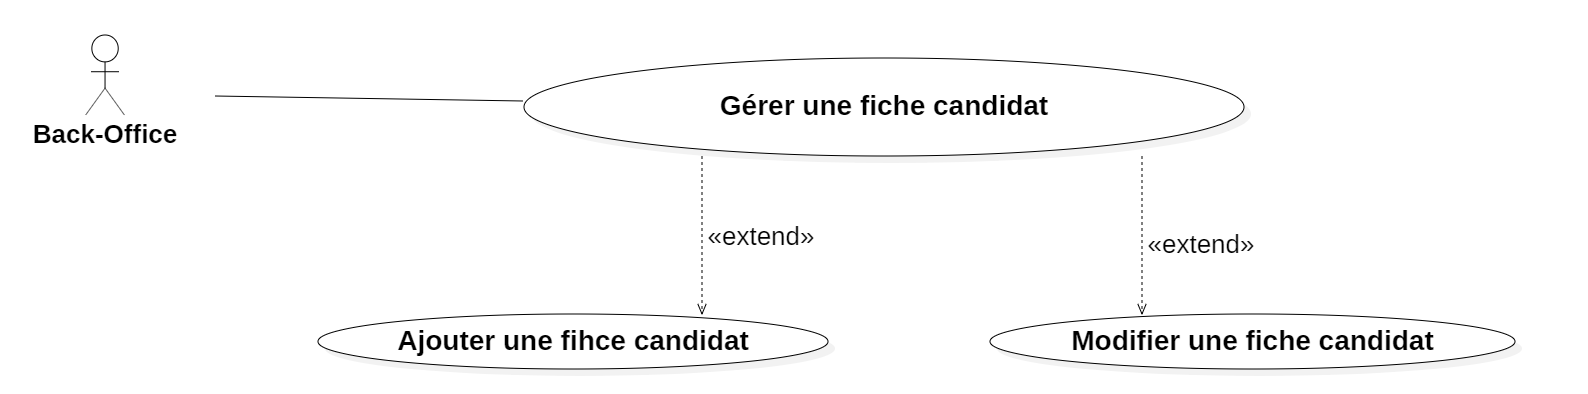
\includegraphics[scale=0.35]{img/raffinement fiche candidat.png}
     \caption{Diagramme de cas d'utilisation "Gérer une fiche candidat"}
     \label{fig:raffinement_fiche_candidat}
 \end{figure}
Nous détaillons dans ce qui suit les deux cas d'utilisation : "Ajouter une fiche candidat" et "Modifier une fiche candidat". Après authentification, le back-office peut toujours créer une nouvelle fiche candidat.
\begin{longtable}[c]{
    |p{.20\textwidth}|
    |p{.70\textwidth}|
}
    \hline
    \textbf{Titre}
    &    Ajouter une fiche candidat\\
    \hline
    \textbf{Résumé}
    & Le back-office peut ajouter une nouvelle fiche candidat. \\
    \hline
     \textbf{Pré-condition}
    & Le back-office doit être authentifié.\\
    \hline
     \textbf{Scénario normal}
    & \begin{itemize}
        \item A1 : Le back office clique sur le bouton "Ajouter fiche candidat".
        \item A2 : Le système affiche le formulaire à remplir.
        \item A3 : Le back-office introduit les informations nécessaires.
        \item A4 : Le système vérifie les informations saisies et ajoute le candidat.
    \end{itemize}\\
    \hline
    \textbf{Enchaînement d'erreur}
    & E1 : Le système affiche un message d'erreur mentionnant la présence d'un champ obligatoire vide.\\
    \hline
    \textbf{Post-condition}
    & Une nouvelle fiche candidat est ajoutée.\\
    \hline
\caption{Description du cas d'utilisation "Ajouter une fiche candidat"}
\label{tab:desc_ajout_fiche}
\end{longtable} 
\newpage
Le back-office peut aussi modifier une fiche candidat.
\begin{longtable}[c]{
    |p{.20\textwidth}|
    |p{.70\textwidth}|
}
    \hline
    \textbf{Titre}
    &    Modifier une fiche candidat\\
    \hline
    \textbf{Résumé}
    & Le back-office peut modifier une fiche candidat déjà créée. \\
    \hline
     \textbf{Pré-condition}
    & Le back-office doit être authentifié.\\
    \hline
     \textbf{Scénario normal}
    & \begin{itemize}
        \item A1 : Une fois la recherche est effectuée, le back office clique sur le bouton "Consulter ou Modifier une fiche candidat" pour le candidat choisis. 
        \item A2 : Le système affiche le formulaire contenant les informations du candidat concerné.
        \item A3 : Le back-office modifie les informations nécessaires.
        \item A4 : Le système vérifie les informations saisies et enregistre les modifications.
    \end{itemize}\\
    \hline
    \textbf{Enchaînement d'erreur}
    & E1 : Le système affiche un message d'erreur mentionnant la présence d'un champ obligatoire vide.\\
    \hline
    \textbf{Post-condition}
    & Une fiche candidat est modifiée.\\
    \hline
\caption{Description du cas d'utilisation "Modifier une fiche candidat"}
\label{tab:desc_modif_fiche}
\end{longtable} 
%%%%%%%%%%%%%%%%%%%%%%%%%%%%%%%%%%%%%%%%%%%%%%%%
\subsubsection{Cas d'utilisation "Gérer un entretien"}
Dans cette partie, nous nous concentrons sur le raffinement du cas d'utilisation "Gérer un entretien". Les fonctionnalités relatives à ce diagramme sont représentées dans la Figure \ref{fig:gerer_entretien}.

\begin{figure}[H]
     \centering
     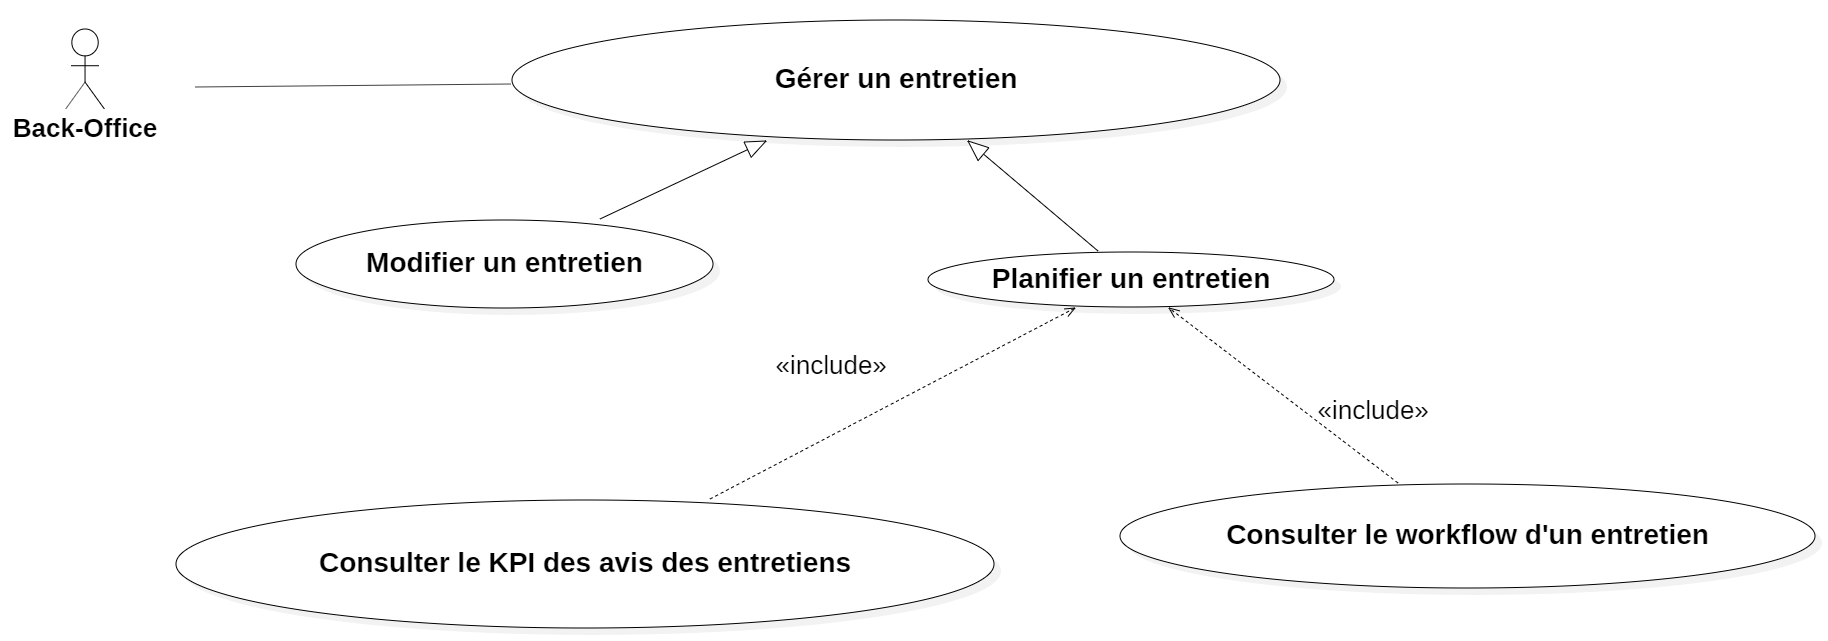
\includegraphics[scale=0.35]{img/raffinement gerer entretien.png}
     \caption{Diagramme de cas d'utilisation "Gérer un entretien"}
     \label{fig:gerer_entretien}
 \end{figure}

Nous détaillons dans ce qui suit les quatres cas d'utilisation : "Planifier un entretien" , "Modifier un entretien", "Consulter le KPI des avis des entretiens" et "Consulter le workflow d'un entretien". Le back-office peut toujours planifier un entretien après avoir été authentifié.
\begin{longtable}[c]{
    |p{.20\textwidth}|
    |p{.70\textwidth}|
}
    \hline
    \textbf{Titre}
    &   Planifier un entretien\\
    \hline
    \textbf{Résumé}
    & Le back-office peut planifier un nouvel entretien. \\
    \hline
     \textbf{Pré-condition}
    & Le back-office doit être authentifié.\\
    \hline
     \textbf{Scénario normal}
    & \begin{itemize}
        \item A1 : Une fois la fiche du candidat est créée, le back-office clique sur le bouton "Planifier un entretien". 
        \item A2 : Le système affiche le formulaire de l'entretien.
        \item A3 : Le back-office introduit les informations nécessaires de l'entretien.
        \item A4 : Le back-office clique sur le bouton "Enregistrer".
        \item A5 : Le système vérifie les informations saisies et ajoute l'entretien.
        \item A6 : Le système attribue le statut "En attente" pour cet entretien.
        \item A7 : Le système envoie un e-mail, généré automatiquement, au recruteur sélectionné, contenant la date, l'heure, les nom et prénom du candidat et un lien qui mène vers la fiche de ce candidat.
    \end{itemize}\\
    \hline
    \textbf{Enchaînement d'erreur}
    & E1 : Le système affiche un message d'erreur mentionnant la présence d'un champ obligatoire vide.\\
    \hline
    \textbf{Post-condition}
    & Un nouvel entretien est ajouté.\\
    \hline
\caption{Description du cas d'utilisation "Planifier un entretien"}
\label{tab:desc_planif_entretien}
\end{longtable} 
Le back-office peut aussi modifier un entretien.
\begin{longtable}[c]{
    |p{.20\textwidth}|
    |p{.70\textwidth}|
}
    \hline
    \textbf{Titre}
    &   Modifier un entretien\\
    \hline
    \textbf{Résumé}
    & Le back-office peut modifier un entretien déjà planifié. \\
    \hline
     \textbf{Pré-condition}
    & Le back-office doit être authentifié.\\
    \hline
     \textbf{Scénario normal}
    & \begin{itemize}
        \item A1 : Une fois un entretien est créé, le back-office clique sur le bouton "Modifier un entretien". 
        \item A2 : Le système affiche le formulaire de l'entretien déjà créé.
        \item A3 : Le back-office introduit les modifications d'informations nécessaires.
        \item A4 : Le back-office clique sur le bouton "Enregistrer".
        \item A5 : Le système vérifie les informations saisies et enregistre les modifications.
    \end{itemize}\\
    \hline
    \textbf{Enchaînement d'erreur}
    & E1 : Le système affiche un message d'erreur mentionnant la présence d'un champ obligatoire vide.\\
    \hline
    \textbf{Post-condition}
    & Un entretien est modifié.\\
    \hline
\caption{Description du cas d'utilisation "Modifier un entretien"}
\label{tab:desc_modif_entretien}
\end{longtable} 

Le back-office peut aussi consulter le KPI des avis des recruteurs lors des entretiens,sachant que ces avis changent d'une implantation à une autre de Talan après qu'un entretien ait été planifié.
\begin{longtable}[c]{
    |p{.20\textwidth}|
    |p{.70\textwidth}|
}
    \hline
    \textbf{Titre}
    &   Consulter le KPI des avis des recruteurs lors des entretiens\\
    \hline
    \textbf{Résumé}
    & Le back-office peut consulter le KPI des avis des entretiens. \\
    \hline
     \textbf{Pré-condition}
    & Le back-office doit être authentifié et l'entretien déjà créé.\\
    \hline
     \textbf{Scénario normal}
    & \begin{itemize}
        \item A1 : Le back-office navigue vers l'interface d'accueil(Dashboard). 
        \item A2 : Le système affiche l'interface contenant un graphe à secteurs montrant le nombre total de candidats par avis(qui concerne l'implantation de Talan du back-office connecté) pour une année sélectionnée au préalable.
    \end{itemize}\\
    \hline
    \textbf{Enchaînement d'erreur}
    & \\
    \hline
    \textbf{Post-condition}
    & Le KPI des avis des entretiens est consulté.\\
    \hline
\caption{Description du cas d'utilisation "Consulter le KPI des avis des entretiens"}
\label{tab:desc_consult_KPI}
\end{longtable} 

Le back-office peut aussi consulter le Workflow d'un entretien qui représente son historique:
\begin{itemize}
    \item \textbf{Au niveau du back-office} : la date de création de l'entretien, les nom et prénom de l'intervenant au back-office qui a créé l'entretien.
    \item \textbf{Au niveau du recruteur} : après l'acceptation ou le rejet de l'entretien par ce dernier : la date de la décision du recruteur, les nom et prénom de celui-ci.
\end{itemize} 
\begin{longtable}[c]{
    |p{.20\textwidth}|
    |p{.70\textwidth}|
}
    \hline
    \textbf{Titre}
    &   Consulter le Workflow d'un entretien\\
    \hline
    \textbf{Résumé}
    & Le back-office peut consulter le workflow d'un entretien déjà créé. \\
    \hline
     \textbf{Pré-condition}
    & Le back-office doit être authentifié et un entretien déjà créé.\\
    \hline
     \textbf{Scénario normal}
    & \begin{itemize}
        \item A1 : Une fois un entretien est créé, le back-office clique sur le bouton "Consulter Workflow" 
        \item A2 : Le système affiche un modal ( Popup: une petite fenêtre) contenant la date de création , les nom et prénom de l'intervenant au back-office qui a créé l'entretien, ainsi que la date de l'acceptation ou du rejet de l'entretien avec le nom et le prénom du recruteur concerné.
    \end{itemize}\\
    \hline
    \textbf{Enchaînement d'erreur}
    & \\
    \hline
    \textbf{Post-condition}
    & La fenêtre du Workflow est affichée.\\
    \hline
\caption{Description du cas d'utilisation "Consulter le workflow d'un entretien"}
\label{tab:desc_consult_workflow}
\end{longtable} 
\subsection{Raffinement des cas d'utilisation pour le recruteur}
Nous développons, dans cette partie, chaque cas d'utilisation du recruteur avec une description détaillée.
\subsubsection{Cas d'utilisation "Valider un entretien"}
Nous nous intéressons, dans cette partie, au raffinement du cas d'utilisation "Valider un entretien". Les fonctionnalités relatives à ce diagramme sont représentées dans la Figure \ref{fig:valid_entretien}
\begin{figure}[H]
     \centering
     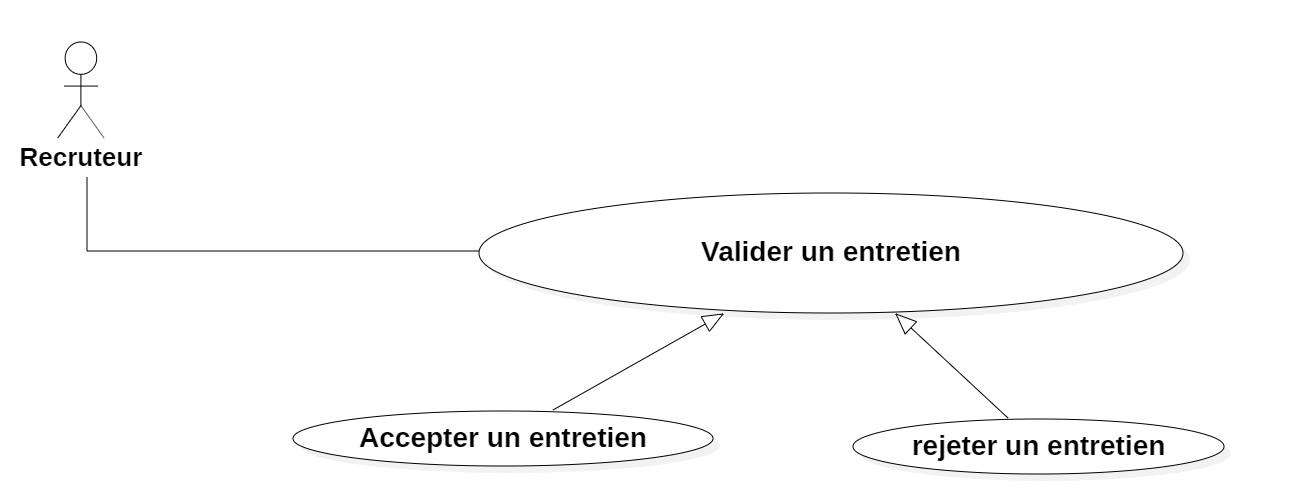
\includegraphics[scale=0.35]{img/raffinement valider un entretien.png}
     \caption{Diagramme de cas d'utilisation "Valider un entretien"}
     \label{fig:valid_entretien}
 \end{figure}
 Nous détaillons dans ce qui suit les deux cas d'utilisation : "Accepter un entretien" et "Rejeter un entretien". Après la planification d'un entretien et l'authentification du recruteur, un e-mail généré automatiquement sera envoyé à ce dernier pour lui notifier qu'un entretien est prévu à une date et à une heure précises, et lui transmettre un lien vers la fiche du candidat sur laquelle il indique sa décision d'accepter ou de rejeter l'entretien.
 \begin{longtable}[c]{
    |p{.20\textwidth}|
    |p{.70\textwidth}|
}
    \hline
    \textbf{Titre}
    &   Accepter un entretien\\
    \hline
    \textbf{Résumé}
    & Le recruteur peut accepter un entretien déjà créé. \\
    \hline
     \textbf{Pré-condition}
    & Le recruteur doit être authentifié et un entretien déjà créé.\\
    \hline
     \textbf{Scénario normal}
    & \begin{itemize}
        \item A1 : Une fois un entretien est créé et l'e-mail est envoyé, le recruteur clique sur le lien dans l'e-mail et l'interface de la fiche du candidat sera chargée. 
        \item A2 : le recruteur clique sur le bouton "Accepter un entretien".
        \item A3 : Le système modifie le statut de l'entretien de "En attente" en "Accepté".
    \end{itemize}\\
    % \hline
    % \textbf{Enchaînement d'erreur}
    % & \\
    \hline
    \textbf{Post-condition}
    & Le statut de l'entretien est modifié en "Accepté"\\
    \hline
\caption{Description du cas d'utilisation "Accepter un entretien"}
\label{tab:accept_entretien}
\end{longtable}
 Le recruteur peut aussi rejeter un entretien.
 \newpage
  \begin{longtable}[c]{
    |p{.20\textwidth}|
    |p{.70\textwidth}|
}
    \hline
    \textbf{Titre}
    &   Rejeter un entretien\\
    \hline
    \textbf{Résumé}
    & Le recruteur peut rejeter un entretien déjà créé. \\
    \hline
     \textbf{Pré-condition}
    & Le recruteur doit être authentifié et un entretien déjà créé.\\
    \hline
     \textbf{Scénario normal}
    & \begin{itemize}
        \item A1 : Une fois un entretien est créé et l'e-mail est envoyé, le recruteur clique sur le lien dans l'e-mail et l'interface de la fiche du candidat sera chargée. 
        \item A2 : le recruteur clique sur le bouton "Rejeter un entretien".
        \item A3 : Le système modifie le statut de l'entretien de "En attente" en "Rejeté".
    \end{itemize}\\
    %\hline
    % \textbf{Enchaînement d'erreur}
    % & \\
    \hline
    \textbf{Post-condition}
    & Un e-mail est envoyé au back-office pour le notifier.\\
    \hline
\caption{Description du cas d'utilisation "Rejeter un entretien"}
\label{tab:rejet_entretien}
\end{longtable}
%%%%%%%%%%%%%%%%%%%%%%%%%%%%%%%%%%%%%%%%%%%%%%%
\subsubsection{Cas d'utilisation "Rechercher un candidat"}
Dans cette partie, nous nous intéressons au raffinement du cas d'utilisation "Rechercher un candidat". Les fonctionnalités relatives à ce diagramme sont représentées dans la figure \ref{fig:recherche_candidat}.
\begin{figure}[H]
     \centering
     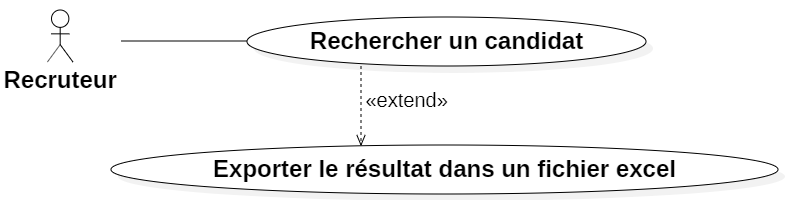
\includegraphics[scale=0.6]{img/raffinement recherche candidat.png}
     \caption{Diagramme de cas d'utilisation "Rechercher un candidat"}
     \label{fig:recherche_candidat}
 \end{figure}
 Nous détaillons dans ce qui suit le cas d'utilisation "Exporter le résultat dans un fichier excel". Après que le recruteur ait effectué une recherche des candidats, le résultat est affiché sous forme d'un tableau. Le recruteur peut sélectionner un ou plusieurs candidats dans le tableau, et clique sur le bouton "Exporter" pour télécharger un fichier excel qui contient toutes les informations concernant les candidats sélectionnés. 
 \newpage
   \begin{longtable}[c]{
    |p{.20\textwidth}|
    |p{.70\textwidth}|
}
    \hline
    \textbf{Titre}
    &   Exporter le résultat dans un fichier excel\\
    \hline
    \textbf{Résumé}
    & Le recruteur peut exporter le résultat de la recherche de candidats dans un fichier excel. \\
    \hline
     \textbf{Pré-condition}
    & Le recruteur doit être authentifié et une recherche doit être effectuée.\\
    \hline
     \textbf{Scénario normal}
    & \begin{itemize}
        \item A1 : Une fois la recherche est effectuée, le recruteur sélectionne le(s) candidat(s) en cliquant sur la case à cocher pour chaque candidat. 
        \item A2 : le recruteur clique sur le bouton "Exporter".
        \item A3 : Le système génère un fichier excel contenant toutes les informations relatives aux candidats sélectionnés, et le télécharge à travers le navigateur .
    \end{itemize}\\
    % \hline
    % \textbf{Enchaînement d'erreur}
    % & \\
    %
    \hline
    \textbf{Post-condition}
    & Un fichier excel est téléchargé.\\
    \hline
\caption{Description du cas d'utilisation "Exporter le résultat dans un fichier excel"}
\label{tab:recherche_candidat}
\end{longtable}
\section*{Conclusion}
Dans ce chapitre, nous avons mis en évidence les acteurs, ainsi que les besoins fonctionnels et non fonctionnels du système.
D'autre part, nous avons détaillé les différents cas d'utilisation en précisant une description textuelle pour chaque cas. En effet, ce chapitre nous a permis de mieux comprendre les fonctionnalités à développer. L'étape suivante concerne la conception de notre application qui sera présenté dans le prochain chapitre.

